\section{Charging and Discharging Capacitors (RC circuits)}

\instructornote{%
By Matt Trawick, 2008, added to manual in 2015.  Time: 50 minutes

This lab assumes that students have built circuits before, and know how to use digital multimeters, for instance.

Equipment notes: 

The values of resistors and capacitors used here are not an accident.  The RC time constants used are slow enough to be easily visible and measurable by the students.  Also, the resistance values are low enough that they are safely below the ~1 Mohm input impedance of the pasco  boxes.   That pushes the capacitors to fairly high values, and you can run into troubles there if the capacitors have a high leakage current.  For this reason, it's important to use capacitors with a reasonably low leakage.  
}

\makelabheader %(Space for student name, etc., defined in master.tex)

\bigskip
\textbf{Apparatus}

\begin{itemize}[nosep]
\item Digital multimeters (2) 
\item DC power supply 
\item Resistors: 10 k$\Omega$ and 27 k$\Omega$
\item Capacitors: 470 $\mu$F and 1000 $\mu$F (``low leakage'')
\item 4 dual banana connectors for resistors and capacitors
\item DPST knife switch with banana jack connectors
\item About six connecting wires
\item Pasco 550 interface, with voltage probe
\item \textit{Capstone} software (\filename{RC\_circuits.cap} experiment file)
\end{itemize}

\bigskip
\textbf{Activity 1: What's happening?}

Build the circuit shown in the diagram below.  The switch terminal labeled ``2'' in the diagram is the center terminal on your switch.

\begin{minipage}{0.82\textwidth}
\begin{newboxed}
%\vspace{-0.2 in}
\textit{Be sure to connect the “negative” end of the capacitor to the negative terminal of the power supply, or it may explode and hurt you.  The negative end of the capacitor is marked with a long stripe down the side of the capacitor with negative signs (``$-$'') on it.  Ask your instructor for help if you are not sure.}
%\vspace{-0.1 in}
\end{newboxed}
\end{minipage}
\begin{minipage}{0.17\textwidth}
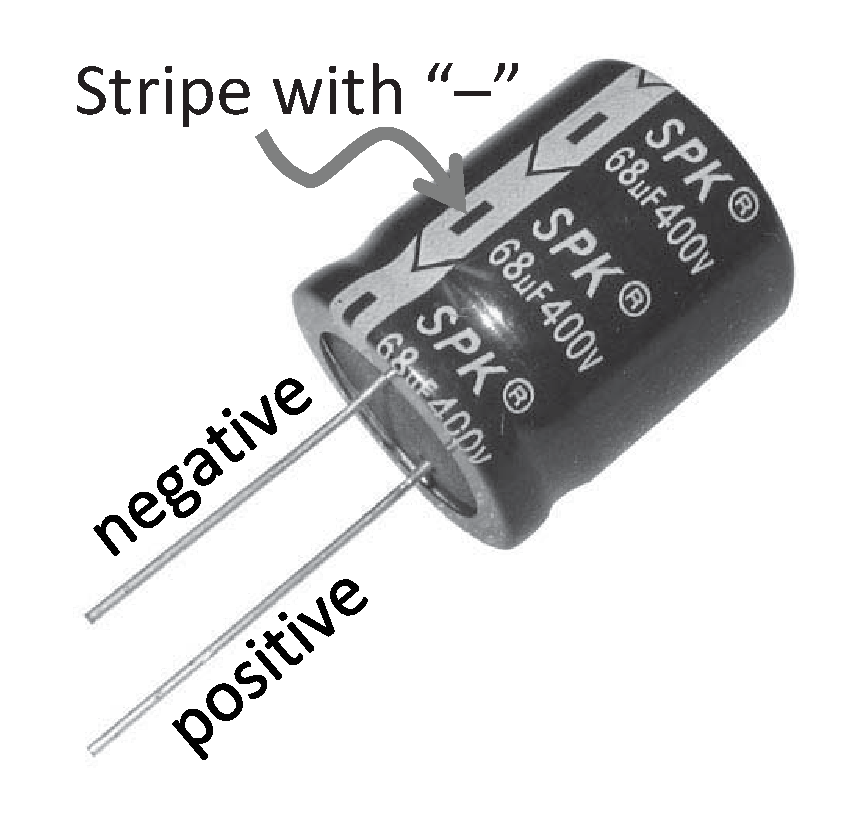
\includegraphics[width=1.0\textwidth]{rc_circuits/capacitor2_bw.eps}
\end{minipage}

\begin{center}
\vspace{-0.3 in}
%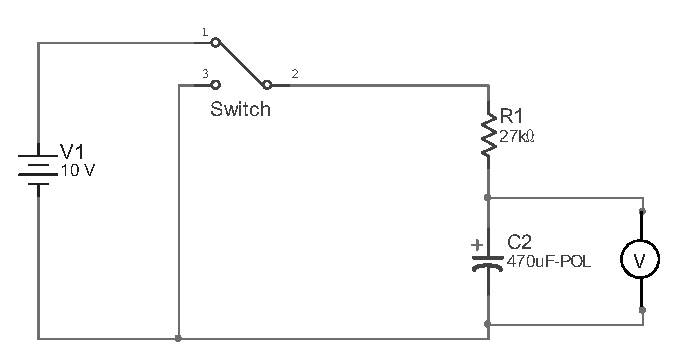
\includegraphics[width=0.6\textwidth]{rc_circuits/circuit_diagram_bw.eps}
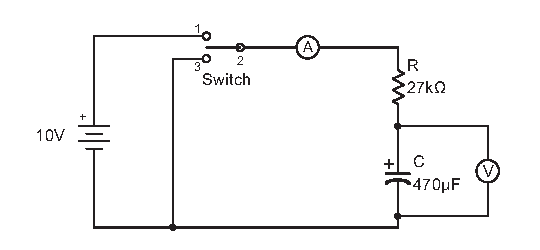
\includegraphics[width=0.6\textwidth]{rc_circuits/single_dc_capacitor3.eps}
\vspace{-0.1 in}
\end{center}

(a) When you move the switch to position ``1,'' so that terminals 1 and 2 are connected, what happens to the voltage difference $\Delta V_C$ across the capacitor?
\answerspace{0.6in}

(b)  With the switch in position ``1,'' what is happening to the charge $Q$ stored on the capacitor?
\answerspace{0.6in}

(c)  Now move the switch to position ``3,'' so that terminals 2 and 3 are connected.  What happens to the voltage difference $\Delta V_C$ and the charge $Q$ on the capacitor?
\answerspace{0.7in}

\pagebreak[2]
(d) Starting with $\Delta V_C$ near zero, (say $\Delta V_C \lesssim 1$~V) move the switch to position ``1'' (charging) and observe the current $I$ measured by your DMM.  (You'll need to set your DMM to a low current scale.)  As the capacitor's charge increases, does the current you measure increase, decrease, or remain constant?
\answerspace{0.5in}

(e) Once the capacitor has been charged (say $\Delta V_C \gtrsim 9$~V) move the switch to position ``3'' (discharging).  Is the sign of the current on your meter the same as in part (d), or is it different?  What is the physical meaning of the sign?
\answerspace{0.7in}

\textbf{Activity 2: Drawing graphs}

Because the voltage $\Delta V_C$ is changing, it will be useful to use your computer to graph $\Delta V_C$ \textit{vs.} time.  Connect the red and black leads of the ``voltage sensor'' (really just an overpriced adapter) from the 550 interface box to the same place in your circuit where your digital voltmeter is connected.  You can keep the DMM plugged in too.
To record voltage versus time data, open the file \filename{RC\_circuits.cap} in the \filename{\coursefolder} folder.

(a)  Now take some data.  On the axes below, draw sketches below showing $\Delta V_C$ \textit{vs.} time starting when the switch is moved into position ``1'' (charging) and position ``3'' (discharging).  Include a scale on the vertical axis.

%\vspace{1.5in}
%\begin{center}
%\vspace{-0.4 in}
%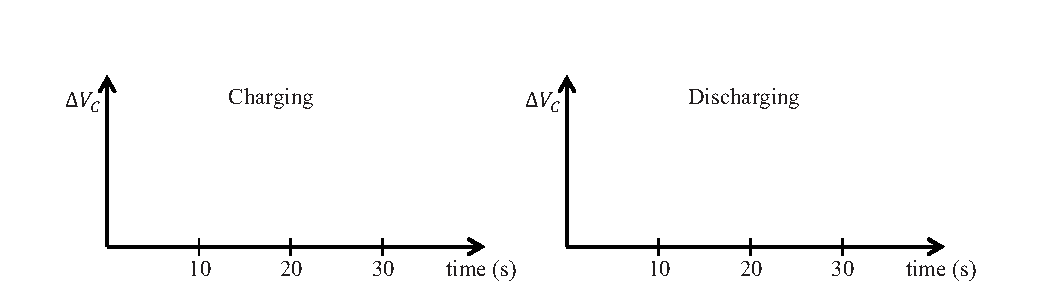
\includegraphics[width=0.95\textwidth]{rc_circuits/vc_axes.eps}
%\vspace{-0.1 in}
%\end{center}

\begin{lab_groupplot}*{}[lab_noticks_1quad,
	group style={
		group size= 2 by 1},
	height=1in,width=2.5in,
	xmin=0,xmax=43,
	xtick={10,20,30},
	title=Charging,
	title style={anchor = north},
	algebraic_labels,
	xlabel=Time (s),
	ylabel=$\Delta V_C$,
]
\nextgroupplot[title=Charging]
\nextgroupplot[title=Discharging]
\end{lab_groupplot}


(b) Repeat the experiment above, this time focusing on the current measured by your DMM.  On the axes below, draw sketches below showing $I$ \textit{vs.} time when the capacitor is charging and discharging.  Include a scale on the vertical axis, and pay attention to the sign.

%\begin{center}
%\vspace{-0.3 in}
%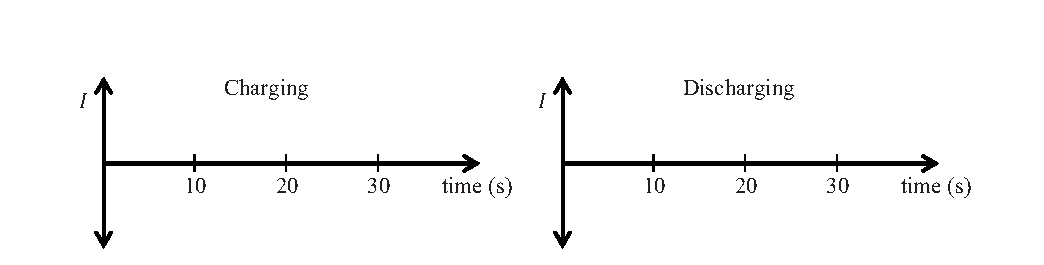
\includegraphics[width=0.95\textwidth]{rc_circuits/current_axes.eps}
%%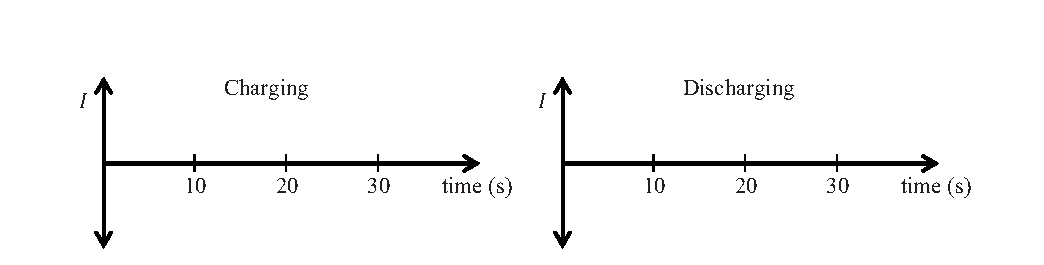
\includegraphics[width=0.6\textwidth]{rc_circuits/current_axes.eps}
%\vspace{-0.1 in}
%\end{center}

\begin{lab_groupplot}*{}[lab_noticks_2quads,
	group style={
		group size= 2 by 1},
	height=1.2in,width=2.5in,
	xmin=0,xmax=43,
	xtick={10,20,30},
	title=Charging,
	title style={anchor = north},
	algebraic_labels,
	xlabel=Time (s),
	ylabel=\hspace*{15.71pt}$I$,  %See calculation below
]
\nextgroupplot[title=Charging]
\nextgroupplot[title=Discharging]
\end{lab_groupplot}

%  \newlength{\myl}
%  \settowidth{\myl}{$I$}
%  \the\myl
%  \settowidth{\myl}{$\Delta V_C$}
%  \the\myl


\begin{wrapfigure}[5]{r}{0.17\textwidth}
    \vspace{-0.2 in}

\includegraphics[width=0.07\textwidth]{rc_circuits/shorted_resistor_bw.eps}
\end{wrapfigure}


(c)  Helpful hint: if you get tired of waiting forever for $\Delta V_C$ to rise and fall, you can briefly ``short out'' the resistor by connecting an additional wire across it, as shown to the right.  
How does ``shorting out'' the resistor affect $\Delta V_C$ when the capacitor is charging?  When the capacitor is discharging?
\answerspace{0.7in}

\pagebreak[2]
\textbf{Activity 3: Measuring the time constant}

(a) Start with the capacitor fully charged at about 10 volts.  Then (with the resistor not shorted out) move the switch to position “3” to discharge the capacitor.  How long does it take for $\Delta V_C$ to drop to 1/3 of its original level (that is, from 10 volts to about 3.3 volts)?
\vspace{0.8in}

(b) If you repeat part (a) with a resistance $R = 10$ k$\Omega$ how do you expect your result to change?  Make a prediction and then test it.

\vspace{0.2 in}
\hspace{0.4 in} Prediction:
\vspace{0.2 in}

\hspace{0.4 in} Measurement:  
\vspace{0.2 in}

%\pagebreak
(c) Go back to using the 27 k$\Omega$ resistor.  Now, if you repeat part (a) with a capacitance of $C=1000$ $\mu$F, how do you expect your result to change?  Make a prediction and then test it.

\vspace{0.2 in}
\hspace{0.4 in} Prediction:
\vspace{0.2 in}

\hspace{0.4 in} Measurement:  
\vspace{0.2 in}

(d) The time it takes for $\Delta V_C$ to fall to about a third of its original value (actually to $1/e$ of its value, where $e=2.71828…$) is called the time constant, $\tau$.   Fill in the following table:

%For fixed width columns:
%These are now defined in master.text, to avoid  warnings when the definition is repeated in each file.
%columntype{L}[1]{>{\raggedright\arraybackslash}p{#1}}
%\newcolumntype{C}[1]{>{\centering\arraybackslash}p{#1}}
%\newcolumntype{R}[1]{>{\raggedleft\arraybackslash}p{#1}}

\vspace{0.1 in}
\hspace*{0.5in}
%\begin{tabular}{|c | c| >{\centering}m{1in} |}
{\renewcommand{\arraystretch}{1.8}
\begin{tabular}{|c | c| C{1in} |}
\hline
$R$ & $C$ & $\tau$ \\ 
\hhline{|=|=|=|}
10 k$\Omega$ & 470 $\mu$F &\\ \hline
27 k$\Omega$ & 470 $\mu$F &\\ \hline
10 k$\Omega$ & 1000 $\mu$F &\\ \hline
27 k$\Omega$ & 1000 $\mu$F &\\ \hline
\end{tabular}
}
\vspace{0.2in}

(e) What is the mathematical relationship between $R$, $C$, and $\tau$? Write a single equation that relates the three.
\vspace{0.7in}

(f) Looking at your graphs, what is the functional form of $\Delta V_C$ \textit{vs.} time  for a discharging capacitor?  Try moving your data to Excel and fitting it to test your hypothesis.
\vspace{0.7in}
